\documentclass[tikz]{standalone}
%\usetikzlibrary{calc}
\begin{document}
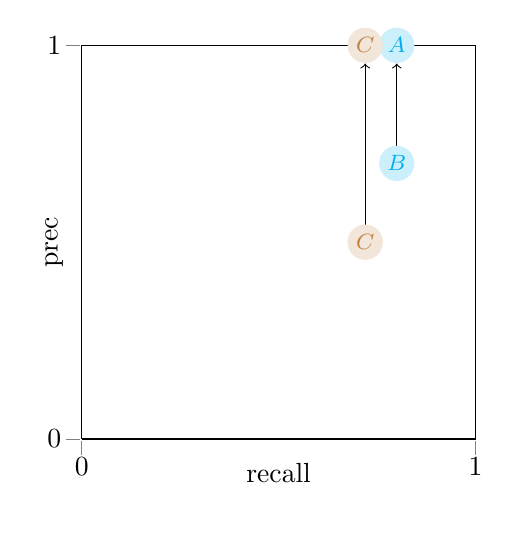
\begin{tikzpicture}[every node/.style={circle, inner sep=0pt}]
\coordinate (SW) at (0,0);
\coordinate (NW) at (0,5);
\coordinate (SE) at (5,0);
\coordinate (NE) at (5,5);

\draw (SW) -- (NW) -- (NE) -- (SE) -- (SW);
\path (SW) -- node[rotate=90, anchor=south] {prec} (NW);
\path (SW) -- node[anchor=north] {recall} (SE);

\begin{scope}[pin distance=5pt]
\node[pin=below:0] at (SW) {};
\node[pin=below:1] at (SE) {};
\node[pin=left:0] at (SW) {};
\node[pin=left:1] at (NW) {};
\end{scope}

\coordinate (A1) at (2.6, 4.5);
\coordinate (B1) at (2.1, 4.5);
\coordinate (C1) at (1.3, 4.5);

\coordinate (A2) at (3.5, 3.5);
\coordinate (B2) at (4.0, 3.5);
\coordinate (C2) at (2.75, 3.5);

\coordinate (A3) at (4.05, 2.5);
\coordinate (B3) at (4.70, 2.5);
\coordinate (C3) at (3.6, 2.5);


\footnotesize
\begin{scope}[every node/.style={circle, inner sep=0pt, minimum size=1.5em, cyan, fill=cyan!20!white}]
\path (NW -| B2) node (B2f) {\(A\)};
\path[->] (B2) edge (B2f);

\end{scope}

\begin{scope}[every node/.style={circle, inner sep=0pt, minimum size=1.5em, brown, fill=brown!20!white}]
\path (NW -| C3) node (C3f) {\(C\)};
\path[->] (C3) edge (C3f);
\end{scope}

%\draw[dotted] (A1) -- (A1 -| NW);
%\draw[dotted] (B2) -- (B2 -| NW);
%\draw[dotted] (C3) -- (C3 -| NW);

\footnotesize

\begin{scope}[every node/.style={circle, inner sep=0pt, minimum size=1.5em, cyan, fill=cyan!20!white}]
\node at (B2) {\(B\)};
\end{scope}

\begin{scope}[every node/.style={circle, inner sep=0pt, minimum size=1.5em, brown, fill=brown!20!white}]
\node at (C3) {\(C\)};
\end{scope}




\end{tikzpicture}
\end{document}
